\section{Problem Set 3 - 22 February 2026}
\subsection{Problem 1 - Toric Code: Warmup}
As discussed in lecture, an example of a topological code is the toric code. We can visualize the physical qubits and stabilizers for the $n=18$ toric code via the following interactive diagram (drag to rotate, scroll or use the toolbar to zoom). Edges of the lattice represent physical qubits, blue dots (on vertices of the lattice) represent $X$ stabilizers, and orange dots (on faces) represent $Z$ stabilizers. \\

How many logical qubits are encoded by this code? 2 - this is because there are 2 non-contractable loops. \\
$Z$ operators applied on the red edges (4,5,6) correspond to a logical operator for this code. This is true. \\
Applying $Z$ operators to the red edges (4,5,6) is a distinct operation from applying $Z$ operators to the green edges $(10,11,12)$. This is true.



\newpage
\subsection{Problem 2 - The Toric Code: Syndrome Measurements}
As previously mentioned, the topology and error correction properties of topological codes are closely related. One way to build intuition for this is to examine how syndromes are corrected for in practice. When asked to give a list of stabilizer generators which anticommute with the error (i.e., syndrome measurements), provide your answer as a list of stabilizer indices. 

Assume there are $Z$ errors on the qubits associated with red edges in the following diagrams. For the one in the top left, these are qubits (5, 6, 13); top right, (8, 9, 16); bottom, (5, 6, 10, 11, 12, 13). \\

Measuring a stabilizer corresponding to a face (orange dot) will reveal an error has occurred in any of the above: this is false. \\

Syndrome indices for the top left diagram: \\
Syndrome indices for the top right diagram: \\
Syndrome indices for the bottom diagram: \\



\newpage
\subsection{Problem 3 - Decoherence free spaces and stabilizers}
Quantum error correction is an example of “active" error correction where one first detects whether an error occurs and then applies a correcting operation. An interesting area of research in quantum information is the possibility of “passive" error correction. We explore in this problem one of these possibilities, Decoherence Free Subspaces (DFS), in the context of stabilizer codes.

Recall the following: If $S$ is the stabilizer for the code $C$, then $\forall V \in S$, and $\forall \ket{\psi} \in C$, $V\ket{\psi = \ket{\psi}}$.

As an example, consider the three qubit bit flip code, $C_{bf}$, where $\ket{0_L} = \ket{000}$ and $\ket{1_L} = \ket{111}$. The stabilizer $S$ is generated by $ZZI$ and $IZZ$, that is $S = \langle ZZI, IZZ \rangle$ 

The code can correct error $E$ if $E$ is a Pauli group element which anticommutes with at least one of the generators of the code.  
 
Give the stabilizer generators which anticommute with each of the following errors.
\begin{itemize}
    \item $E_1 = XII$, then $S = \langle ZZI\rangle$
    \item $E_1 = IXI$, then $S = \langle ZZI, IZZ\rangle$
    \item $E_1 = IIX$, then $S = \langle IZZ\rangle$
    \item $E_4 = ZIZ$, then $S = \emptyset$
\end{itemize}




\newpage
\subsection{Problem 4 - Topological QEC - A Projective Plane Code}
Quantum error correction codes can be constructed using graphs on topological surfaces, where vertices and faces correspond to certain stabilizer operations, and the distance of the code is given by the shortest non-trivial topological chain of errors. In this problem, we explore a specific instance of such a construction, on a projective plane. \\

The projective plane in two dimensions, $\mathfrak{R}P^2$, can be drawn as a disc in which antipodal points on the boundary are identified. Recall that a cellulation $\mathcal{C}$ of a surface defines sets $F$, $E$, and $V$ of faces, edges, and vertices. For each $e \in E$, there corresponds a qubit on which $X_e$ and $Z_e$ are the Pauli $X$ and $Z$ operators. Let $E_f \subset E$ be the set of edges around face $f \in F$, and let $E_v \subset E$ be the set of edges attached to vertex $v \in V$. For the set of all $f$ and $v$, we define
\begin{align}
    A_f &= \bigotimes\limits_{e \in E_f} Z_e \\
    B_v &= \bigotimes\limits_{e \in E_v} X_e \\
\end{align}
The set of all $A_f$ and $B_v$ is the stabilizer for the code. We want to find a list of stabilizers for the following (three $A_f$ and single unique $B_v$ for the cellulation: 

\begin{center}
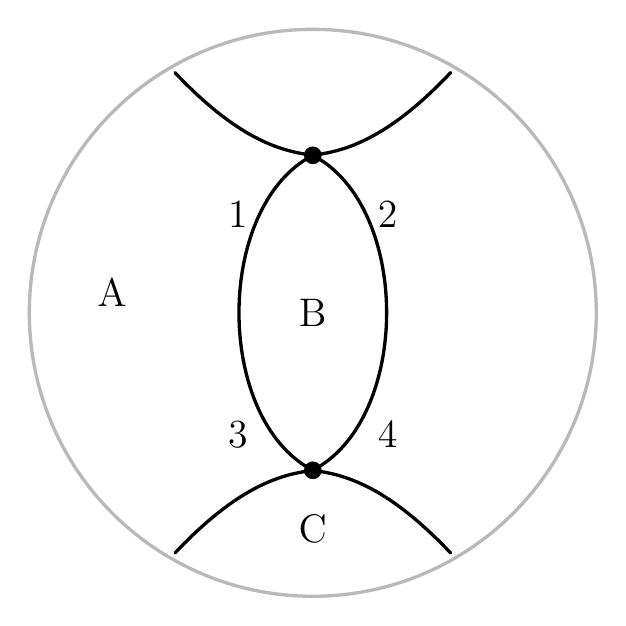
\begin{tikzpicture}[scale=1, line cap=round, line join=round]

% --- Parameters (adjust to taste) ---
\def\R{3.6}        % outer radius
\def\ytop{2.0}     % y of top black dot
\def\ybot{-2.0}    % y of bottom black dot
\def\xbulge{1.25}  % half-width of the B-oval

% --- Outer circle ---
\draw[gray!55, line width=1.2pt] (0,0) circle (\R);

% --- Top cap boundary curve (a smooth arc) ---
\draw[line width=1.2pt]
  (-1.75,3.05)
  .. controls (-0.9,2.15) and (-0.35,2.05) .. (0,\ytop)
  .. controls (0.35,2.05) and (0.9,2.15) .. (1.75,3.05);

% --- Central region B boundary (vertical oval made of two Beziers) ---
\draw[line width=1.2pt]
  (0,\ytop)
  .. controls (-\xbulge,1.35) and (-\xbulge,-1.35) .. (0,\ybot);
\draw[line width=1.2pt]
  (0,\ytop)
  .. controls (\xbulge,1.35) and (\xbulge,-1.35) .. (0,\ybot);

% --- Bottom cap boundary curve (a smooth arc) ---
\draw[line width=1.2pt]
  (-1.75,-3.05)
  .. controls (-0.9,-2.15) and (-0.35,-2.05) .. (0,\ybot)
  .. controls (0.35,-2.05) and (0.9,-2.15) .. (1.75,-3.05);

% --- Black nodes (dots) ---
\fill (0,\ytop) circle (3.2pt);
\fill (0,\ybot) circle (3.2pt);

% --- Labels ---
\node at (-2.55,0.25) {\Large A};
\node at (0,0.0)      {\Large B};
\node at (0,-2.75)    {\Large C};

% --- Edge numbers ---
\node at (-0.95,1.25) {\Large 1};
\node at ( 0.95,1.25) {\Large 2};
\node at (-0.95,-1.55){\Large 3};
\node at ( 0.95,-1.55){\Large 4};

\end{tikzpicture}
\end{center}


This code acts on four qubits ($|E| = 4$), corresponding to the four edges, labeled $1$ through $4$. Note there are only three distinct faces, labeled $A$, $B$, and $C$. These stabilizers must commute with each other.\\

There are 3 face stabilizers: \\
\begin{itemize}
    \item For face A: $ZZZZ$
    \item For face B: $ZZII$
    \item For face C: $IIZZ$
\end{itemize}
There are 2 vertices, however they both give the same stabilzer: $XXXX$ \\
Therefore the stabilizers are:
\begin{equation}
    [ZZZZ,ZZII,IIZZ,XXXX]
\end{equation}



\newpage
\subsection{Problem 5 - Topological QEC - A Projective Plane Code II}
In problem 4, we want to find out the states that they stabilize. The list of stabilizers from Problem 4 is 
\begin{equation}
    [ZZZZ,ZZII,IIZZ,XXXX]
\end{equation}
Then the states they stabilize are:
\begin{align}
    \ket{0_L} = \ket{0000} + \ket{1111} \\
    \ket{0_L} = \ket{0011} + \ket{1100} 
\end{align}


\newpage
\subsection{Problem 6 - Topological QEC - Another Projective Plane Code}
Quantum error correction codes can be constructed using graphs on topological surfaces, where vertices and edges correspond to certain stabilizer operations, and the distance of the code is given by the shortest non-trivial topological chain of errors. In this problem, we explore a specific instance of such a construction, on a projective plane.\\

The projective plane in two dimensions, $\mathfrak{R}P^2$, can be drawn as a disc in which antipodal points on the boundary are identified. Recall that a cellulation $\mathcal{C}$ of a surface defines sets $F$, $E$, and $V$ of faces, edges, and vertices. For each $e \in E$, there corresponds a qubit on which $X_e$ and $Z_e$ are the Pauli $X$ and $Z$ operators. Let $E_f \subset E$ be the set of edges around face $f \in F$, and let $E_v \subset E$ be the set of edges attached to vertex $v \in V$. For the set of all $f$ and $v$, we define
\begin{align}
    A_f &= \bigotimes\limits_{e \in E_f} Z_e \\
    B_v &= \bigotimes\limits_{e \in E_v} X_e \\
\end{align}
The set of all $A_f$ and $B_v$ is the stabilizer for the code. We want to find a list of stabilizers for the following cellulation:

\begin{center}
    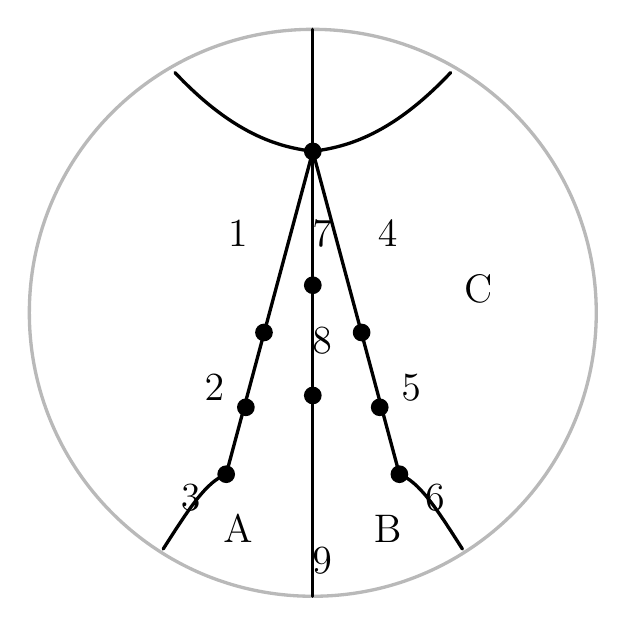
\begin{tikzpicture}[scale=1, line cap=round, line join=round]

% ----------------- Parameters (tweak to match perfectly) -----------------
\def\R{3.6}          % outer radius
\def\ytop{2.05}      % y-position of the apex dot
\def\capx{1.75}      % half-width of the top cap arc endpoints (x)
\def\capy{3.05}      % y of the top cap arc endpoints

% Key points
\coordinate (O)    at (0,0);
\coordinate (Top)  at (0,\R);
\coordinate (Bot)  at (0,-\R);

\coordinate (P)    at (0,\ytop);         % apex dot
\coordinate (L3)   at (-1.10,-2.05);     % lower-left slanted endpoint (dot)
\coordinate (R6)   at ( 1.10,-2.05);     % lower-right slanted endpoint (dot)

% Intermediate dots on slanted edges
\coordinate (L2)   at (-0.85,-1.20);
\coordinate (L1)   at (-0.62,-0.25);
\coordinate (R5)   at ( 0.85,-1.20);
\coordinate (R4)   at ( 0.62,-0.25);

% Dots on the center vertical line
\coordinate (C7)   at (0,0.35);
\coordinate (C8)   at (0,-1.05);

% Bottom arc endpoints (where the small arcs meet the outer circle)
\coordinate (BL)   at (-1.90,-3.00);
\coordinate (BR)   at ( 1.90,-3.00);

% ----------------- Outer circle -----------------
\draw[gray!55, line width=1.2pt] (O) circle (\R);

% ----------------- Top cap arc + top vertical segment -----------------
\draw[line width=1.2pt]
  (-\capx,\capy)
  .. controls (-0.95,2.20) and (-0.35,2.10) .. (P)
  .. controls ( 0.35,2.10) and ( 0.95,2.20) .. (\capx,\capy);

% vertical line from top of circle to apex
\draw[line width=1.2pt] (Top) -- (P);

% ----------------- Central vertical line (down to bottom) -----------------
\draw[line width=1.2pt] (P) -- (Bot);

% ----------------- Slanted boundaries -----------------
\draw[line width=1.2pt] (P) -- (L3);
\draw[line width=1.2pt] (P) -- (R6);

% ----------------- Bottom curved arcs (A and B boundaries) -----------------
\draw[line width=1.2pt]
  (BL) .. controls (-1.55,-2.45) and (-1.35,-2.15) .. (L3);
\draw[line width=1.2pt]
  (BR) .. controls ( 1.55,-2.45) and ( 1.35,-2.15) .. (R6);

% ----------------- Dots -----------------
\foreach \pt in {P,L1,L2,L3,R4,R5,R6,C7,C8}
  \fill (\pt) circle (3.2pt);

% ----------------- Region labels -----------------
\node at (-0.95,-2.75) {\Large A};
\node at ( 0.95,-2.75) {\Large B};
\node at ( 2.10, 0.30) {\Large C};

% ----------------- Edge/segment numbers -----------------
\node at (-0.95, 1.00) {\Large 1};
\node at (-1.25,-0.95) {\Large 2};
\node at (-1.55,-2.35) {\Large 3};

\node at ( 0.95, 1.00) {\Large 4};
\node at ( 1.25,-0.95) {\Large 5};
\node at ( 1.55,-2.35) {\Large 6};

\node at ( 0.12, 1.00) {\Large 7};
\node at ( 0.12,-0.35) {\Large 8};
\node at ( 0.12,-3.15) {\Large 9};

\end{tikzpicture}
\end{center}

For the 3 faces: Face A: $A_1 = ZZZIIIZZZ$, Face B: $A_2 = IIIZZZZZZ$, Face C: $A_3 = ZZZZZZIII$

For the 7 vertices:
\begin{itemize}
    \item Vertex 7: $B_1 = XIXXIXXIX$
    \item Vertex 1: $B_2 = XXIIIIIII$, Vertex 3: $B_3 = IXXIIIIII$
    \item Vertex 4: $B_4 = IIIXXIIII$, Vertex 6: $B_5 = IIIIXXIII$
    \item Vertex 8: $B_6 = IIIIIIXXI$, Vertex 9: $B_7 = IIIIIIIXX$
\end{itemize}



\newpage
\subsection{Problem 7 - Topological QEC - Another Projective Plane Code II}
The dimension of the vector space stabilized by these stabilizers is given by $2^{n-m}$. Here $n = 9$. We want to find the number of independent stabilizer generators. \\

There are 3 faces $A$, $B$, $C$, hence 3 operators $A_f$, but they satisfy $A_AA_BA_C = I$ because every edge appears in the boundary of exactly two faces (so every $Z_e$ appears twice and cancels). Therefore the number of independent face stabilizers is: 3-1 = 2 \\

There are 9 vertices, but from the  antipodal identification
\begin{itemize}
    \item 1 top vertices (edges 1,4,7 meet)
    \item 2 vertices on the left branch (one between edges 1-2, and one between edges 2-3)
    \item 2 vertices on the right branch (one between edges 4-5, and one between edges 5-6)
    \item 2 vertices on the central branch (one between edges 7-8, and one between edges 8-9)
\end{itemize}
Therefore we have 7 vertices. But the satisfy $B_1 B_2\cdots B_7 = I$. Therefore, the number of independent vertex stabilizers is $7-1=6$. \\

Therefore there are a total of $m$ independent stabilizers. \\

The dimension of the vector space stabilzed by these stabilizers is then given by $2^{9-8} = 2$. 


\newpage
\subsection{Problem 8 - Toric code on $3x3$ lattice}
Recall that the toric code had stabilizer generators
\begin{equation}
    B_f = \prod_{e\sim f} Z_e \text{ and } A_v = \prod_{e\sim v} X_e
\end{equation}
for faces $f$ and vertices $v$. Measuring these generators produces the syndromess, and once syndromes of the code are measured, we may process this data using classical routines to determine the recovery operation needed to be applied to fix errors. However, there is a great deal of flexibility in the classical routine we choose! In this problem, we will explore one such routine for the toric code and analyze its performance in a random error model. \\

We study a toric code on a $3\times 3$ square lattice. Define coordinates for the vertices so that $(0,0)$ is the bottom left vertex. Label coordiates for the faces so that $(1/2, 1/2)$ is the bottom face: 

\begin{center}
    \begin{tikzpicture}[scale=1.35, line cap=round, line join=round]

% --- Axes ---
\draw[-{Stealth[length=3mm,width=2mm]}, gray!70, line width=0.9pt] (0,0) -- (3.05,0);
\draw[-{Stealth[length=3mm,width=2mm]}, gray!70, line width=0.9pt] (0,0) -- (0,3.05);

% --- Dotted guide lines (as in the picture) ---
\draw[gray!55, dotted, line width=0.9pt] (1,0) -- (1,3);  % x=1
\draw[gray!55, dotted, line width=0.9pt] (2,0) -- (2,3);  % x=2
\draw[gray!55, dotted, line width=0.9pt] (0,1) -- (3,1);  % y=1
\draw[gray!55, dotted, line width=0.9pt] (0,2) -- (3,2);  % y=2

% --- Points (blue) ---
\tikzset{pt/.style={circle, fill=blue!85!black, draw=blue!85!black, inner sep=0pt, minimum size=7pt}}

% x = 0 column: y = 1/2, 3/2, 5/2
\node[pt] at (0,0.5) {};
\node[pt] at (0,1.5) {};
\node[pt] at (0,2.5) {};

% x = 1/2 column: y = 0,1,2
\node[pt] at (0.5,0) {};
\node[pt] at (0.5,1) {};
\node[pt] at (0.5,2) {};

% x = 1 column: y = 1/2, 3/2, 5/2
\node[pt] at (1,0.5) {};
\node[pt] at (1,1.5) {};
\node[pt] at (1,2.5) {};

% x = 3/2 column: y = 0,1,2
\node[pt] at (1.5,0) {};
\node[pt] at (1.5,1) {};
\node[pt] at (1.5,2) {};

% x = 2 column: y = 1/2, 3/2, 5/2
\node[pt] at (2,0.5) {};
\node[pt] at (2,1.5) {};
\node[pt] at (2,2.5) {};

% x = 5/2 column: y = 0,1,2
\node[pt] at (2.5,0) {};
\node[pt] at (2.5,1) {};
\node[pt] at (2.5,2) {};

% --- Tick labels (fractions like the figure) ---
% x-axis labels at 0, 1/2, 1, 3/2, 2, 5/2
\node[gray!70] at (0,-0.28) {$0$};
\node[gray!70] at (0.5,-0.28) {$\frac12$};
\node[gray!70] at (1,-0.28) {$1$};
\node[gray!70] at (1.5,-0.28) {$\frac32$};
\node[gray!70] at (2,-0.28) {$2$};
\node[gray!70] at (2.5,-0.28) {$\frac52$};

% y-axis labels at 0, 1/2, 1, 3/2, 2, 5/2
\node[gray!70, anchor=east] at (-0.18,0) {$0$};
\node[gray!70, anchor=east] at (-0.18,0.5) {$\frac12$};
\node[gray!70, anchor=east] at (-0.18,1) {$1$};
\node[gray!70, anchor=east] at (-0.18,1.5) {$\frac32$};
\node[gray!70, anchor=east] at (-0.18,2) {$2$};
\node[gray!70, anchor=east] at (-0.18,2.5) {$\frac52$};

\end{tikzpicture}
\end{center}



Note that we also identify the top and bottom edges and the left and right edges to form a 2-torus, and recall that qubits (depicted as blue dots in the above figure) are positioned on edges.

\begin{enumerate}
    \item Syndrome operators are associated with a vertex or a face. Suppose the error $X_{(1/2,0)} \otimes Y_{(1,1/2)} \otimes Y_{1,3/2} \otimes Z_{2,3/2}$ happens. Which syndrome operators anticommute with this error? Give a list of the vertices and faces corresponding to these syndrome operator. \\

    We look for faces touching edges with $X$ or $Y$. 
    \begin{itemize}
        \item Horizontal edge (1/2,0) touches faces: (1/2, 1/2) and (1/2,5/2)
        \item Vertical edge (1,1/2) touches faces (1/2, 1/2) and (3/2,1/2) 
        \item Vertical edge (1,3/2) touches faces (1/2, 3/2) and (3/2, 3/2)
    \end{itemize}

    Now we count parity by face: 
    \begin{itemize}
        \item Face (1/2, 1/2) touches (1/2,0)$\rightarrow X$ and (1,1/2)$\rightarrow Y$; That is 2 X-components, an even number which means it commutes
        \item Face (1/2, 5/2) touches (1/2, 0) $\rightarrow 1 \rightarrow$ anticommutes
        \item Face (3/2, 1/2) touches (1,1/2) $\rightarrow 1 \rightarrow$ anticommutes
        \item Face (1/2, 3/2) touches (1,3/2) $\rightarrow 1 \rightarrow$ anticommutes
        \item Face (3/2, 3/2) touches (1,3/2) $\rightarrow 1 \rightarrow$ anticommutes
    \end{itemize}
    Therefore, the 4 face syndromes are $[(1/2,5/2), (3)]$
\end{enumerate}




\newpage
\subsection{Problem 9 - Syndrome decoding for random errors - recovery}




\newpage
\subsection{Problem 10 - Syndrome decoding for random errors - correctness}




\newpage
\subsection{Problem 11 - Matching algorithm performance}




\newpage
\subsection{Problem 12 - Matching algorithm performance II}




\newpage
\subsection{Problem 13 - Matching algorithm performance III}